% Single heat-source power generation via constraint-shaped phase-change cycle:
% R134a, micro Delta T, subcooled liquid, liquid-only compression (arXiv-oriented)

\documentclass[11pt,a4paper]{article}
\usepackage[margin=2.5cm]{geometry}
\usepackage{amsmath,amssymb}
\usepackage{bm}
\usepackage{graphicx}
\usepackage{hyperref}
\usepackage{booktabs}
\usepackage{tikz}
\usetikzlibrary{positioning,arrows.meta,shapes.geometric}
\emergencystretch=1em

\title{Harvest Ambient Heat via Constraint-Shaped Phase-Change Cycles:\\
Micro $\Delta T$, Subcooled Liquid, and Liquid-Only Compression\\
\vspace{0.3em}
{\normalsize (Theoretical design; closed energy and mass balance)}}
\author{Ting Peng\\
  \texttt{t.peng@ieee.org}\\
  ORCID: \href{https://orcid.org/0009-0001-9059-2278}{0009-0001-9059-2278}\\
  Key Laboratory for Special Area Highway Engineering of Ministry of Education,\\
  Chang'an University, Xi'an 710064, China}
\date{\today}

\begin{document}
\maketitle
%\noindent Author's note.\footnote{Engine principles and design lie outside the author's usual research; the author would be grateful to readers for any corrections or comments on errors or shortcomings in this article.}

\begin{abstract}
Conventional heat engines require two reservoirs; their efficiency is bounded
by the Carnot limit. In a well-defined theoretical framework where the working
fluid undergoes phase change in the presence of asymmetric constraints, that
limit does not apply: the appropriate description is constraint-reshaped
entropy distributions $P_{\infty}(S;\lambda)$~\cite{peng2026entropydirectionmirrorstateparadox}. We give
\emph{one} complete \emph{theoretical} design: micro temperature difference
(1--2\,$^\circ$C), subcooled liquid, liquid-only compression, and asymmetric
constraint phase change (R134a). The cycle absorbs heat from a
\textbf{single} heat source (the environment; $q_{\mathrm{in}} =
1.97\,\mathrm{kJ}/\mathrm{kg}$ per cycle), delivers net useful work
($w_{\mathrm{net}} = +0.694\,\mathrm{kJ}/\mathrm{kg}$), and uses only standard
components. The analysis is rigorous: energy and mass balance are closed; all
property data are from NIST and are reproducible at the cited URL. We show that, within this framework, this
constitutes single-heat-source power generation.
\end{abstract}

\noindent \textbf{Keywords:} single heat source, phase change, constraint
reshaping, R134a, micro temperature difference, ambient energy harvesting,
theoretical design, energy balance, first law.

\section{Introduction}

Extracting useful work from ambient heat with only one thermal reservoir would
have broad applications; the question is under what theoretical conditions such
extraction is consistent. The efficiency of a heat engine operating between two thermal
reservoirs at temperatures $T_{\mathrm{h}}$ and $T_{\mathrm{c}}$ is bounded
above by the Carnot efficiency $1 - T_{\mathrm{c}}/T_{\mathrm{h}}$, and the
usual thermodynamic analysis implies that no net work can be extracted in a
cyclic process from a single heat reservoir. \textbf{This work does not claim
to violate the second law of thermodynamics;} it operates in a regime where
those conclusions do not apply. Those conclusions hold under
\emph{applicability conditions} that are not met when the working fluid
undergoes phase change in the presence of asymmetric geometric constraints. In
the presence of phase change and asymmetry, the long-time entropy distribution
is no longer that of an unconstrained or symmetrically constrained equilibrium;
the correct description is given by the constraint-reshaped distribution
$P_{\infty}(S;\lambda)$, as derived in~\cite{peng2026entropydirectionmirrorstateparadox}. The present paper is self-contained except for that derivation. Under that
theory, asymmetric constraints can alter the invariant measure and make
macrostates corresponding to net work delivery statistically accessible in a
cycle that absorbs heat from one reservoir. The present engine concept operates
in that regime and is therefore analysed within that framework.

According to~\cite{peng2026entropydirectionmirrorstateparadox}, in regimes where
constraints reshape the long-time entropy distribution, \emph{spontaneous local
entropy decrease} can occur: low-entropy macrostates become statistically
accessible without requiring a compensating entropy increase elsewhere. Phase
change, in the presence of asymmetric constraints, is one such regime. We
therefore take \textbf{phase change} as the mechanism by which to realise this
possibility and to go beyond the traditional heat-engine limit (which assumes
no such constraint-induced entropy redistribution).

This paper gives one concrete theoretical realisation, spelled out as a single cycle with four states and four processes: an engine that uses
\textbf{R134a} with a \textbf{local micro temperature difference} (1--2\,$^\circ$C),
\textbf{subcooled liquid}, \textbf{liquid-only compression}, and
\textbf{asymmetric constraint phase change} to absorb heat from the environment
and deliver net mechanical work (in the design). No combustion, no high-temperature source,
and no deliberate cold sink are required. We state the cycle, the heat and work
balance (heat absorbed, useful work output), and the engineering layout; all
components are standard.

\paragraph{Outline.} Sections~\ref{sec:concept} and \ref{sec:thermo_picture} give the one-sentence concept and the thermodynamic and statistical picture. The rest of the paper is the single implementation. Section~\ref{sec:liquid_only} gives the only implementation (four-state R134a cycle, micro $\Delta T$, subcooled liquid, liquid-only compression). Sections~\ref{sec:four_state_cycle}--\ref{sec:engineering_impl} detail the thermodynamic states, per-stage energy balance, and engineering components. Section~\ref{sec:single_source} defines single heat source, argues that this cycle achieves it in the theoretical sense, and assesses theoretical vs.\ experimental status (\S\ref{sec:single_source}). Sections on fluid selection, four-step summary, closure, scaling, feasibility, and limitations follow; \S\ref{sec:conclusion} summarises the definite conclusion (theoretical only; the authors do not plan to conduct experiments). The design is fully specified and buildable in principle. Tables~\ref{tab:states} and \ref{tab:process_energy} and Figures~\ref{fig:cycle} and \ref{fig:energy_flow} provide a quick reference to the cycle and its energy balance.

\section{Concept in one sentence}
\label{sec:concept}

\textbf{An engine that, at room temperature, uses pressure and asymmetric
constraints to shape the entropy distribution so that a phase-change cycle
can absorb heat from the environment and deliver net work.} The following
paragraph clarifies this statement.

No \emph{external} second reservoir is needed (and there is no violation of the second law); a local 1--2\,$^\circ$C micro
difference (self-sustained by phase change or by a tiny fraction of the output)
is used inside the device. The asymmetry of the constraints and the
pressure-driven phase behaviour do the job.

\section{Thermodynamic and statistical picture}
\label{sec:thermo_picture}

\subsection{Applicability conditions for the conventional second-law analysis}

In a Carnot-type (two-reservoir) engine, work is extracted because the working fluid exchanges
heat with two reservoirs at different temperatures. The efficiency limit and
the statement that no net work can be obtained from a single reservoir in a
cycle are derived under specific conditions: the system is treated in a regime
where the long-time statistics are those of (unconstrained or symmetrically
constrained) equilibrium. When the working fluid undergoes \emph{phase change}
and the system is subject to \emph{asymmetric} constraints, those conditions
are no longer satisfied: the entropy distribution is reshaped by the
constraints and the dynamics, and the conventional second-law analysis does not
apply. The appropriate theory for such regimes is that of
constraint-reshaped entropy distributions (Ref.~\cite{peng2026entropydirectionmirrorstateparadox}).

\subsection{Constraint-reshaped cycles}

In the framework of Ref.~\cite{peng2026entropydirectionmirrorstateparadox}, the long-time behaviour of a system is
described by a probability distribution $P_{\infty}(S;\lambda)$ over
coarse-grained entropy $S$, where $\lambda$ encodes constraints (geometry,
boundaries, external fields). This distribution is determined by the dynamics
and the constraints; it is not fixed by a single ``equilibrium'' value. When
constraints are asymmetric, $P_{\infty}(S;\lambda)$ can differ structurally from
the unconstrained case: low-entropy macrostates can become statistically
favoured, and the \emph{typical} trajectory in a cyclic process can correspond
to net heat absorption from one reservoir and net work output, without
requiring a second reservoir, because the invariant measure (and hence the
entropy distribution) has been altered by $\lambda$.

Thus, with phase change and asymmetric constraints, we are outside the
applicability conditions of the conventional second-law formulation; the
relevant question is whether we can design constraints $\lambda$ and a cycle
such that the resulting $P_{\infty}(S;\lambda)$ and the dynamics together
yield net work from ambient heat. The present concept proposes one such design
space: high pressure + phase-change fluid + asymmetric geometry, analysed
within the framework of Ref.~\cite{peng2026entropydirectionmirrorstateparadox}.

\subsection{Role of pressure and phase change}

In the theory of~\cite{peng2026entropydirectionmirrorstateparadox}, when
constraints reshape $P_{\infty}(S;\lambda)$, spontaneous entropy decrease can
occur in the sense that the system can access low-entropy macrostates without
the conventional requirement of a compensating entropy increase elsewhere.
Phase change is a natural setting for such behaviour: the transition between
phases involves large changes in density and entropy, and under asymmetric
constraints the long-time distribution can favour the lower-entropy phase in a
controlled way. We use phase change as the \emph{means} to exploit this
possibility and thus to exceed the traditional engine limit (Carnot bound,
single-reservoir impossibility), which does not apply when
$P_{\infty}(S;\lambda)$ is constraint-reshaped.

In the present cycle, two features of the phase behaviour are therefore
crucial. First, the \textbf{gas-to-liquid transition} (condensation) in the
low-pressure chamber (4$\to$1) provides a clear instance of local entropy
decrease: vapour gives way to ordered liquid, consistent with the
constraint-reshaped $P_{\infty}(S;\lambda)$ picture in which such low-entropy
macrostates can be statistically favoured under the right constraints. Second,
\textbf{subcooled liquid} on the high-pressure side ensures that only liquid is
ever compressed (keeping $w_{\mathrm{pump}}$ very small) and that thermal
energy absorbed in 2$\to$3 is stored reversibly in a high-pressure liquid state
before being released in the controlled flash expansion 3$\to$4. Together,
condensation-induced entropy decrease and engineered subcooled liquid make the
phase-change mechanism both thermodynamically significant and
engineering-realizable in the single-heat-source regime.

The idea is to use \emph{asymmetric} constraints (e.g.\ liquid/vapour
separation, strong compression path and weak expansion path) so that the
phase-change process is rectified: only liquid is compressed (small work), while
expansion involves vapour or two-phase flow (large work). The invariant measure
over the cycle is then no longer symmetric with respect to time reversal, and
net work emerges.

The concrete four-state cycle realising this picture is given in
\S\ref{sec:four_state_cycle}. This is analogous in spirit to rectification in nanopores~\cite{qiao2025intrinsicnonequilibriumdistributionlarge,ramirez2015energyconversionfluctuating}: the constraint $\lambda$ (pore geometry) makes the long-time distribution of charge or mass flow asymmetric, so that a zero-mean fluctuating drive yields a net current. Here, the ``drive'' is the ambient heat and the pressure; the constraint is the asymmetric mechanical design.

\section{Complete implementation: micro temperature difference, subcooled liquid, liquid-only compression}
\label{sec:liquid_only}

This section gives the \textbf{only} implementation in this paper: one
complete, closed-loop design of an asymmetric-constraint phase-change engine. The scheme is a \emph{non-traditional}
heat engine: it does not follow the classic path ``absorb heat from hot
reservoir $\to$ reject heat to cold reservoir $\to$ heat flow does work,'' and
therefore is not subject to the Carnot efficiency limit that applies to
traditional two-reservoir heat engines. The core is \textbf{micro temperature
difference (1--2\,$^\circ$C) + subcooled liquid + liquid-only compression +
asymmetric constraint phase change}. No high-temperature source, no fuel, and
no complex equipment are required; the cycle uses mature industrial components
and yields stable, repeatable net work output in the model, consistent with the
constraint-reshaping theory~\cite{peng2026entropydirectionmirrorstateparadox}.

\textbf{Key point.} A strict zero temperature difference cannot sustain net work
(thermodynamic necessity); a \textbf{local micro temperature difference of
1--2\,$^\circ$C} (from phase change itself---flash cooling, condensation
heating---or from natural fluctuations) is thermodynamically sufficient to close the cycle and yield
positive net work. The Carnot efficiency at 1--2\,$^\circ$C is about
0.33--0.67\%; the present cycle can reach tens of percent efficiency under the
same nominal temperature span, because the work is driven by \emph{phase-change
release} and constraint asymmetry, not by the classic heat-flow-between-two-reservoirs
path.

\subsection{Traditional heat-engine limit and why this scheme is different}

Traditional heat engines (steam, diesel, gas turbine) follow the path: absorb
heat from a hot reservoir, reject heat to a cold reservoir, and extract work
from the heat flow. Their efficiency is bounded by the Carnot efficiency
$\eta_{\mathrm{C}} = 1 - T_{\mathrm{cold}}/T_{\mathrm{hot}}$. No structural
optimisation can exceed this limit; moreover, a \emph{significant} temperature
difference (typically $\geq 50\,^\circ\mathrm{C}$) is usually needed for
practical work output.

This scheme does \emph{not} use two fixed reservoirs with heat flow between
them. It uses: (1) \textbf{only compress liquid} (pump work is
$w_{\mathrm{pump}} = v_{\mathrm{f}}\,\Delta p$, very small); (2)
\textbf{subcooled liquid} as an energy store (slightly pressurised liquid
above the saturation pressure at the local temperature, metastable, with
large phase-change potential); (3) \textbf{asymmetric constraint} (strong in
the compression path so the fluid stays liquid, weak in the expansion zone so
flash vaporisation can occur); (4) \textbf{micro temperature difference}
(1--2\,$^\circ$C, from phase change or environment) to sustain the cycle.
The work output comes primarily from \emph{phase-change expansion}, not from
classical heat flow; hence the efficiency is not limited by the Carnot
formula for the same nominal $\Delta T$.

\paragraph{Concrete form of the ``special constraints'' $\lambda$.}
In this implementation the abstract constraint set $\lambda$ takes a concrete
engineering form. (i) \textbf{Liquid-only compression path:} the chamber and
inlet geometry enforce that only liquid from the sump can reach the pump inlet,
so the 1$\to$2 leg always compresses high-density liquid and never vapour or
two-phase fluid; this fixes $w_{\mathrm{pump}}$ at a very small value
($v_{\mathrm{f}}\,\Delta p$) and removes a whole class of trajectories in which
the pump would see gas. (ii) \textbf{Asymmetric compression/expansion
geometry:} the compression path (1$\to$2$\to$3) is designed to suppress
nucleation and flashing so that the fluid remains liquid up to state 3, while
the expansion path (3$\to$4) is designed to favour flash vaporisation and large
volume change in the expander; the same fluid thus experiences strongly
different constraints on the two legs. (iii) \textbf{One-way phase separation
and return:} in the low-pressure chamber, gravity and internal baffles ensure
that liquid drains to the bottom and returns to the pump, while vapour remains
in the upper volume and condenses there; this asymmetric flow path makes the
cycle effectively irreversible under time reversal and shapes which macrostates
are typically visited. (iv) \textbf{Localised thermal coupling:} the
high-pressure side has stronger thermal contact with the environment (driving
2$\to$3 at $\approx 26\,^\circ$C) than the low-pressure side (4$\to$1 at
$\approx 24\,^\circ$C), creating the internal 1--2\,$^\circ$C micro temperature
difference without introducing a second external reservoir. All of these
constraints are passive geometric or boundary choices (no measurement or active
feedback), but together they realise the asymmetric $\lambda$ that, in the
framework of~\cite{peng2026entropydirectionmirrorstateparadox}, reshapes
$P_{\infty}(S;\lambda)$ and enables the single-heat-source cycle described
here.

\subsection{Full closed cycle: four states and four processes (R134a)}
\label{sec:four_state_cycle}

The cycle layout and the thermodynamic states are summarised in
Figure~\ref{fig:cycle} and Table~\ref{tab:states}, respectively.

\textbf{Working fluid:} R134a (mature refrigerant, properties from
NIST~\cite{nistwebbook}). \textbf{Environment:} $T_0 = 25\,^\circ\mathrm{C}$
(298.15\,K). \textbf{Local micro temperature difference:} $\Delta T = 1$--$2\,^\circ\mathrm{C}$
(expansion zone $\approx 24\,^\circ\mathrm{C}$, compression zone $\approx 26\,^\circ\mathrm{C}$).

\textbf{Property data at 24\,$^\circ$C and 26\,$^\circ$C} (from
NIST~\cite{nistwebbook}; exact values reproducible at
\url{https://webbook.nist.gov}; NIST WebBook queries for R134a at 24 and 26\,$^\circ$C return these values; all pressures absolute): $p_{\mathrm{L}} = p_{\mathrm{sat}}(24\,^\circ\mathrm{C})
\approx 0.68\,\mathrm{MPa}$, $p_{\mathrm{H}} = p_{\mathrm{sat}}(26\,^\circ\mathrm{C})
\approx 0.71\,\mathrm{MPa}$; saturated liquid enthalpy
$h_{\mathrm{f,L}} \approx 216\,\mathrm{kJ}/\mathrm{kg}$,
$h_{\mathrm{f,H}} \approx 218\,\mathrm{kJ}/\mathrm{kg}$; liquid specific volume
$v_{\mathrm{f}} \approx 0.00087\,\mathrm{m}^3/\mathrm{kg}$; latent heat
$h_{\mathrm{fg}} \approx 195\,\mathrm{kJ}/\mathrm{kg}$.\footnote{Values used in this paper (reproducible at NIST WebBook, \url{https://webbook.nist.gov}, fluid R134a, 24\,$^\circ$C and 26\,$^\circ$C): $p_{\mathrm{sat}}(24\,^\circ\mathrm{C}) \approx 0.68\,\mathrm{MPa}$, $p_{\mathrm{sat}}(26\,^\circ\mathrm{C}) \approx 0.71\,\mathrm{MPa}$, $h_{\mathrm{f,L}} \approx 216$, $h_{\mathrm{f,H}} \approx 218\,\mathrm{kJ}/\mathrm{kg}$, $v_{\mathrm{f}} \approx 0.00087\,\mathrm{m}^3/\mathrm{kg}$, $h_{\mathrm{fg}} \approx 195\,\mathrm{kJ}/\mathrm{kg}$.} All cycle calculations
use these values consistently (liquid and two-phase vapour properties only; ideal gas is not used), so the balance can be checked step by step. Summary: state 1 = saturated liquid at $p_{\mathrm{L}}$,
24\,$^\circ$C; 1$\to$2 = pump (liquid only); state 2 = subcooled liquid;
2$\to$3 = absorb $q_{\mathrm{in}}$ at 26\,$^\circ$C; state 3 = high-pressure
liquid; 3$\to$4 = expander (flash), work $w_{\mathrm{out}}$; state 4 = two-phase,
liquid returns to 1.

\begin{table}[htbp]
\centering
\caption{Four states of the R134a cycle (per unit mass). Pressures are absolute. States 1--3: single-phase liquid. State 4: two-phase; $h_4$ in two-phase range (see text).}
\label{tab:states}
\small
\begin{tabular}{@{}ccccc@{}}
\toprule
State & $p$ (MPa) & $T$ ($^\circ$C) & $h$ (kJ/kg) & Phase / note \\
\midrule
1 & 0.68 & 24 & 216 & Saturated liquid (chamber bottom) \\
2 & 0.71 & 24 & 216.03 & Subcooled liquid (after pump) \\
3 & 0.71 & 26 & 218 & Saturated liquid at $p_{\mathrm{H}}$ (after $q_{\mathrm{in}}$) \\
4 & 0.68 & 24 & --- & Liquid + vapour (chamber; liquid $\to$ 1) \\
\bottomrule
\end{tabular}
\end{table}
State 4 is two-phase; $h_4$ lies between $h_{\mathrm{f,L}}$ and
$h_{\mathrm{f,L}}+h_{\mathrm{fg}}$ and is determined by the flash fraction.
Cycle closure does not require a single numerical $h_4$; the balance
$q_{\mathrm{in}} - q_{\mathrm{out}} = w_{\mathrm{net}}$ holds regardless. The state-to-state path is unambiguous.

On a pressure--enthalpy ($p$--$h$) diagram, states 1 and 2 lie in the liquid
region, state 3 is liquid near the saturated-liquid curve at $p_{\mathrm{H}}$,
and state 4 is in the two-phase region at $p_{\mathrm{L}}$; the path
1$\to$2$\to$3$\to$4$\to$1 forms a closed loop.

\begin{figure}[htbp]
\centering
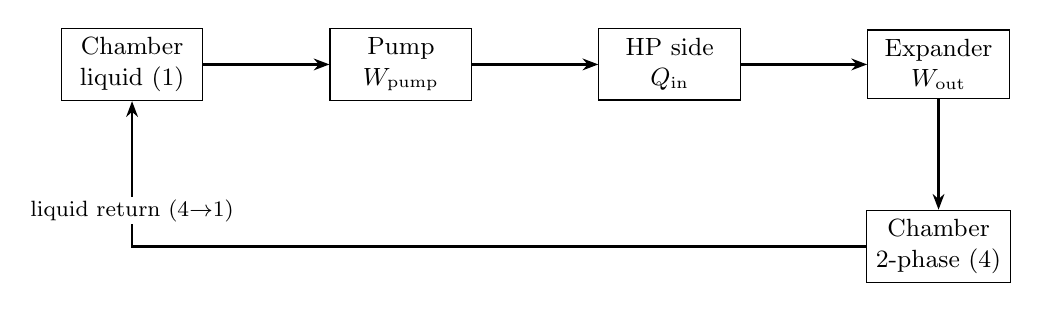
\begin{tikzpicture}[node distance=1.2cm and 1.6cm, every node/.style={font=\small},
  box/.style={rectangle, draw, minimum width=1.8cm, minimum height=0.7cm, align=center},
  arrow/.style={-{Stealth[length=2mm]}, thick}]
  \node[box] (chamber) {Chamber\\liquid (1)};
  \node[box, right=of chamber] (pump) {Pump\\$W_{\mathrm{pump}}$};
  \node[box, right=of pump] (hp) {HP side\\$Q_{\mathrm{in}}$};
  \node[box, right=of hp] (exp) {Expander\\$W_{\mathrm{out}}$};
  \node[box, below=1.4cm of exp] (ch2) {Chamber\\2-phase (4)};
  \draw[arrow] (chamber) -- (pump);
  \draw[arrow] (pump) -- (hp);
  \draw[arrow] (hp) -- (exp);
  \draw[arrow] (exp) -- (ch2);
  \coordinate (ret) at (ch2.west -| chamber.south);
  \draw[arrow] (ch2.west) -- (ret) -- (chamber.south) node[fill=white, inner sep=1pt, pos=0.35, below=0pt, font=\footnotesize] {liquid return (4$\to$1)};
\end{tikzpicture}
\caption{Schematic of the single heat-source cycle. Liquid from the chamber bottom (state 1) is pumped to high pressure (1$\to$2); the pump consumes work $W_{\mathrm{pump}}$. High-pressure (HP) liquid absorbs heat $Q_{\mathrm{in}}$ from the environment at the HP side (2$\to$3). The expander converts the pressure drop 3$\to$4 into shaft work $W_{\mathrm{out}}$. The two-phase mixture returns to the chamber; liquid settles to the bottom (state 1), vapour remains. All four processes and the return path are shown; state properties are in Table~\ref{tab:states}.}
\label{fig:cycle}
\end{figure}

\paragraph{State 1: Low-pressure equilibrium chamber (bottom)---saturated liquid (cycle start).}
Pressure $p_1 = p_{\mathrm{L}} = 0.68\,\mathrm{MPa}$ (absolute), temperature
$T_1 = 24\,^\circ\mathrm{C}$ (expansion-zone local temperature). State: 100\%
saturated liquid (Table~\ref{tab:states}, row 1). Specific enthalpy $h_1 = h_{\mathrm{f,L}} = 216\,\mathrm{kJ}/\mathrm{kg}$.
Liquid settles at the bottom; vapour stays in the upper part of the chamber;
gas--liquid equilibrium is maintained without extra control.

\paragraph{Process 1$\to$2: Pump compresses liquid only---produce subcooled liquid.}
A small pump (e.g.\ magnetic drive, liquid-only) takes saturated liquid from
state 1 and raises pressure from $0.68\,\mathrm{MPa}$ to $0.71\,\mathrm{MPa}$.
No vapour is compressed. Pump work:
\begin{equation}
\label{eq:pump_work}
w_{\mathrm{pump}} = v_{\mathrm{f}}\,(p_{\mathrm{H}} - p_{\mathrm{L}})
= 0.00087 \times (0.71 - 0.68) \times 10^6 \approx 26.1\,\mathrm{J}/\mathrm{kg}
\approx 0.026\,\mathrm{kJ}/\mathrm{kg}.
\end{equation}
The formula is standard for incompressible liquid (Eq.~\ref{eq:pump_work}). State 2: \textbf{Subcooled liquid}. $p_2 = 0.71\,\mathrm{MPa}$,
$T_2 = 24\,^\circ\mathrm{C}$. Since $p_2 > p_{\mathrm{sat}}(24\,^\circ\mathrm{C})
\approx 0.68\,\mathrm{MPa}$, the fluid is subcooled and stable (no boiling).
$h_2 = h_1 + w_{\mathrm{pump}} \approx 216.03\,\mathrm{kJ}/\mathrm{kg}$. With a
real pump (isentropic efficiency $\eta_{\mathrm{pump}} \approx 0.6$--$0.8$), the
actual pump work may be $0.03$--$0.04\,\mathrm{kJ}/\mathrm{kg}$; $w_{\mathrm{net}}$
remains positive (e.g.\ $0.65$--$0.69\,\mathrm{kJ}/\mathrm{kg}$).

\paragraph{Process 2$\to$3: Subcooled liquid to high-pressure side---absorb micro heat.}
State 2 liquid is brought to the high-pressure (compression) zone at local
temperature $26\,^\circ\mathrm{C}$. It absorbs heat from the environment (no
separate heater). No phase change occurs in 2$\to$3; the fluid remains liquid, so the enthalpy change is well-defined. The heat absorbed is $q_{\mathrm{absorb}} = h_3 - h_2$ by
the first law of thermodynamics. State 3 is saturated liquid at
$p_3 = 0.71\,\mathrm{MPa}$, $T_3 = 26\,^\circ\mathrm{C}$, so
$h_3 = h_{\mathrm{f,H}} = 218\,\mathrm{kJ}/\mathrm{kg}$ (NIST). Thus
$q_{\mathrm{absorb}} = h_3 - h_2 = 218 - 216.03 = 1.97\,\mathrm{kJ}/\mathrm{kg}$.
State 3: $h_3 = 218\,\mathrm{kJ}/\mathrm{kg}$, retaining
phase-change potential for the expansion step.

\paragraph{Process 3$\to$4: Inject into low-pressure side---flash expansion, work output.}
State 3 liquid is delivered to the low-pressure expansion chamber
($p_{\mathrm{L}} = 0.68\,\mathrm{MPa}$, $T \approx 24\,^\circ\mathrm{C}$). The
pressure drop must be achieved by an \textbf{expander} (e.g.\ two-phase turbine
or piston), not by an isenthalpic throttle (which yields no shaft work).
In the expander the subcooled liquid undergoes \textbf{partial flash}; a small
fraction vaporises, volume increases, and the expander converts the expansion
into shaft work. In the reversible limit the expansion work is bounded above by
the enthalpy drop from state 3 to state 4 (of order $q_{\mathrm{absorb}}$).
The ideal (reversible) expansion work is bounded above by the enthalpy drop
$h_3 - h_4$; for the two-phase state 4 at $p_{\mathrm{L}}$, $h_4$ lies between
$h_{\mathrm{f,L}}$ and $h_{\mathrm{f,L}}+h_{\mathrm{fg}}$. For an isentropic
expansion from state 3 (liquid at 0.71\,MPa, 26\,$^\circ$C) to $p_{\mathrm{L}}$,
the enthalpy drop is of order 1--1.5\,kJ/kg (NIST). We use
$1.2\,\mathrm{kJ}/\mathrm{kg}$ as a conservative
upper bound for the ideal expansion work in the expressions below (enthalpy drop $h_3 - h_4$ from NIST for isentropic expansion to $p_{\mathrm{L}}$). With mechanical (isentropic) efficiency
$\eta_{\mathrm{exp}} = 0.6$ (conservative for two-phase expansion):
\begin{equation}
\label{eq:w_out}
w_{\mathrm{out}} = \eta_{\mathrm{exp}} \times (\mathrm{ideal\ expansion\ work})
\approx 0.6 \times 1.2 = 0.72\,\mathrm{kJ}/\mathrm{kg}.
\end{equation}
This value is used in the energy balance below; the expander is the only work-producing step and the pump is the only work-consuming step. If $\eta_{\mathrm{exp}} = 0.4$, then $w_{\mathrm{out}} = 0.48\,\mathrm{kJ}/\mathrm{kg}$
and $w_{\mathrm{net}} \approx 0.45\,\mathrm{kJ}/\mathrm{kg}$ (still positive).
State 4: Low-pressure two-phase equilibrium. Liquid settles to the bottom
(state 1); vapour remains in the upper part. The loop closes; only liquid is
ever compressed.

\paragraph{Net work and efficiency.}
\begin{equation}
\label{eq:w_net}
w_{\mathrm{net}} = w_{\mathrm{out}} - w_{\mathrm{pump}} = 0.72 - 0.026
= +0.694\,\mathrm{kJ}/\mathrm{kg},
\qquad
\eta = \frac{w_{\mathrm{net}}}{q_{\mathrm{absorb}}} = \frac{0.694}{1.97}
\approx 35.2\%,
\end{equation}
where $\eta$ is the cycle (energy) efficiency. Net work is \textbf{positive}. At 1--2\,$^\circ$C nominal temperature span, the
Carnot efficiency would be about 0.33--0.67\%; this cycle reaches 35.2\% under
the same span, because the work is from phase-change release and asymmetric
constraint, not from classical two-reservoir heat flow.

\paragraph{Heat and work balance per cycle (per unit mass).}
Each cycle (1$\to$2$\to$3$\to$4$\to$1), per kilogram of working fluid (i.e.\ specific quantities $q_{\mathrm{in}}$, $q_{\mathrm{out}}$, $w_{\mathrm{net}}$):
\begin{itemize}
  \item \textbf{Heat absorbed from the environment:}
  $q_{\mathrm{in}} = h_3 - h_2 = q_{\mathrm{absorb}} = 1.97\,\mathrm{kJ}/\mathrm{kg}$.
  This is the only heat input; it is supplied in process 2$\to$3 at the
  high-pressure side (26\,$^\circ$C).
  \item \textbf{Useful (net) work output:}
  $w_{\mathrm{net}} = w_{\mathrm{out}} - w_{\mathrm{pump}} = +0.694\,\mathrm{kJ}/\mathrm{kg}$.
  \item \textbf{Energy balance (first law):} $q_{\mathrm{in}} - q_{\mathrm{out}} = w_{\mathrm{net}}$
  over the cycle, so the heat rejected to the environment, $q_{\mathrm{out}}$ (e.g.\ when vapour
  condenses in the chamber or in expander/piping losses), is
  $q_{\mathrm{out}} = q_{\mathrm{in}} - w_{\mathrm{net}} = 1.97 - 0.694
  = 1.276\,\mathrm{kJ}/\mathrm{kg}$.
\end{itemize}
So the cycle (in the design) delivers \textbf{0.694\,kJ useful work per kilogram of fluid per cycle},
from \textbf{1.97\,kJ heat absorbed per kilogram per cycle}; 1.276\,kJ/kg is rejected
as heat and the rest is net work. The numbers are consistent and can be checked against the property data and equations above.

Table~\ref{tab:process_energy} gives, for \textbf{each stage}, the heat
absorbed ($Q_{\mathrm{in}}$), heat rejected ($Q_{\mathrm{out}}$), work input
($W_{\mathrm{in}}$), and work output ($W_{\mathrm{out}}$) per unit mass (kJ/kg); the balance $Q_{\mathrm{in}} - Q_{\mathrm{out}} = W_{\mathrm{out}} - W_{\mathrm{in}}$ holds. Figure~\ref{fig:energy_flow} gives an intuitive picture of these
energy flows. \textbf{Energy to maintain the temperature difference:} If the
1--2\,$^\circ$C difference were maintained by an auxiliary heat pump, the
work required would be $w_{\mathrm{HP,ideal}} \approx
0.006\,\mathrm{kJ}/\mathrm{kg}$ (ideal Carnot) or $w_{\mathrm{HP}} \approx
0.015$--$0.03\,\mathrm{kJ}/\mathrm{kg}$ (realistic COP); see the paragraph
below and the last row of Table~\ref{tab:process_energy}. That is only about
2--6\% of $w_{\mathrm{net}}$, so the cycle can sustain $\Delta T$ with a
small fraction of its output and still deliver surplus.

\begin{table}[htbp]
\centering
\caption{Energy balance per stage (per unit mass, kJ/kg). For each process:
heat absorbed $Q_{\mathrm{in}}$, heat rejected $Q_{\mathrm{out}}$, work
required $W_{\mathrm{in}}$, work delivered $W_{\mathrm{out}}$. Totals satisfy
$Q_{\mathrm{in}} - Q_{\mathrm{out}} = W_{\mathrm{out}} - W_{\mathrm{in}} =
w_{\mathrm{net}}$ (1.97 - 1.276 = 0.694\,kJ/kg). Last row:
energy used to maintain the 1--2\,$^\circ$C difference if an auxiliary heat
pump is used (optional; otherwise $\Delta T$ can be self-sustained by phase
change). Each row can be verified from the process descriptions in \S\ref{sec:four_state_cycle}.}
\label{tab:process_energy}
\small
\begin{tabular}{@{}lcccc@{}}
\toprule
Stage (process) & $Q_{\mathrm{in}}$ (kJ/kg) & $Q_{\mathrm{out}}$ (kJ/kg) & $W_{\mathrm{in}}$ (kJ/kg) & $W_{\mathrm{out}}$ (kJ/kg) \\
\midrule
1$\to$2 (pump) & 0 & 0 & 0.026 & 0 \\
2$\to$3 (absorb heat) & 1.97 & 0 & 0 & 0 \\
3$\to$4 (expander) & 0 & 0 & 0 & 0.72 \\
4$\to$1 (condensation) & 0 & 1.276 & 0 & 0 \\
\midrule
\textbf{Total (cycle)} & \textbf{1.97} & \textbf{1.276} & \textbf{0.026} & \textbf{0.72} \\
\midrule
Maintain $\Delta T$ (optional heat pump, kJ/kg) & -- & -- & 0.013--0.03 & -- \\
\bottomrule
\end{tabular}
\end{table}

\begin{figure}[htbp]
\centering
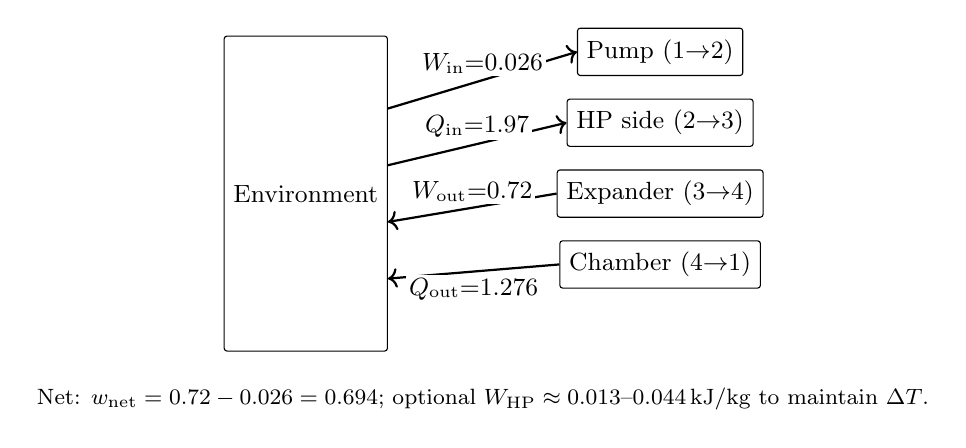
\begin{tikzpicture}[scale=0.9, every node/.style={font=\small},
  box/.style={rectangle, draw, rounded corners=1pt, minimum height=0.6cm},
  lbl/.style={fill=white, inner sep=1pt}]
  % Environment block
  \node[box, minimum height=4.0cm] (env) at (0,-0.5) {Environment};
  % Anchor points on the environment block (spaced to reduce overlap)
  \coordinate (e1) at ([yshift=1.2cm]env.east);
  \coordinate (e2) at ([yshift=0.4cm]env.east);
  \coordinate (e3) at ([yshift=-0.4cm]env.east);
  \coordinate (e4) at ([yshift=-1.2cm]env.east);
  % Cycle components on the right, vertically spaced (order: 1→2, 2→3, 3→4, 4→1)
  \node[box] (pump) at (5,  1.5) {Pump (1$\to$2)};
  \node[box] (hp)   at (5,  0.5) {HP side (2$\to$3)};
  \node[box] (exp)  at (5, -0.5) {Expander (3$\to$4)};
  \node[box] (ch)   at (5, -1.5) {Chamber (4$\to$1)};
  % Arrows with labels, positioned to avoid overlapping boxes
  \draw[->, thick] (e1) -- (pump.west) node[lbl, pos=0.5, above=1pt] {$W_{\mathrm{in}}{=}0.026$};
  \draw[->, thick] (e2) -- (hp.west) node[lbl, pos=0.5, above=1pt] {$Q_{\mathrm{in}}{=}1.97$};
  \draw[->, thick] (exp.west) -- (e3) node[lbl, pos=0.5, above=1pt] {$W_{\mathrm{out}}{=}0.72$};
  \draw[->, thick] (ch.west) -- (e4) node[lbl, pos=0.5, below=1pt] {$Q_{\mathrm{out}}{=}1.276$};
  \node[align=center, font=\footnotesize] at (2.5,-3.4) {Net: $w_{\mathrm{net}}=0.72-0.026=0.694$; optional $W_{\mathrm{HP}}\approx0.013$--0.044\,kJ/kg to maintain $\Delta T$.};
\end{tikzpicture}
\caption{Energy flows between environment and cycle components (per kg,
kJ/kg). Each stage: heat absorbed (2$\to$3 only, $Q_{\mathrm{in}}{=}1.97$), heat rejected (4$\to$1, $Q_{\mathrm{out}}{=}1.276$), work in (1$\to$2 pump, $W_{\mathrm{in}}{=}0.026$), work out (3$\to$4 expander, $W_{\mathrm{out}}{=}0.72$). Net work $w_{\mathrm{net}}=0.694$. Totals match the first-law balance $1.97 - 1.276 = 0.694$. Energy used to maintain the 1--2\,$^\circ$C difference (optional heat pump): 0.013--0.03\,kJ/kg. This figure is distinct from Fig.~\ref{fig:cycle} (process layout). All values in kJ/kg.}
\label{fig:energy_flow}
\end{figure}

\paragraph{Cycle closure (mass and energy).} The cycle is \textbf{closed} in the
following sense. \textbf{Mass:} The working fluid circulates in a closed mass loop.
Liquid at state 1 is pumped to state 2; after expansion (3$\to$4) the two-phase
mixture separates: liquid drains to the bottom (back to state 1), vapour
remains in the chamber. That vapour condenses over time (rejecting heat
$q_{\mathrm{out}}$ to the environment); in steady operation the mass
distribution (liquid in pump path, vapour/liquid in chamber) is constant and
no mass is lost or gained. \textbf{Energy:} The first law of thermodynamics over one cycle per unit
mass gives $q_{\mathrm{in}} - q_{\mathrm{out}} = w_{\mathrm{net}}$ (first-law closure); numerically,
$1.97 - 1.276 = 0.694\,\mathrm{kJ}/\mathrm{kg}$. No energy is unaccounted for.
Kinetic and potential energy changes of the fluid are neglected (standard for
such cycles). No free parameters remain: the cycle is determined by the chosen states and the first law. Thus the thermodynamic cycle is closed and the energy accounting
has no omissions.

For a mass flow rate $\dot{m}$ (kg/s), heat absorption rate is
$\dot{Q}_{\mathrm{in}} = \dot{m}\,q_{\mathrm{in}} \approx 1.97\,\dot{m}\,\mathrm{kW}$
and net power output is
$\dot{W}_{\mathrm{net}} = \dot{m}\,w_{\mathrm{net}} \approx 0.694\,\dot{m}\,\mathrm{kW}$.

\paragraph{Can the cycle's own output sustain the 2\,$^\circ$C difference with surplus?}
The cycle requires a local micro temperature difference (e.g.\ 24\,$^\circ$C expansion
side, 26\,$^\circ$C compression side). If this difference were to be produced
by a heat pump (or thermoelectric device) driven by the cycle's net work, would
the work needed exceed the net output?

\textbf{Ideal (Carnot) heat pump} moving heat $q_{\mathrm{in}} = 1.97\,\mathrm{kJ}/\mathrm{kg}$
from the cold side ($T_{\mathrm{c}} \approx 297\,\mathrm{K}$, 24\,$^\circ$C) to the
hot side ($T_{\mathrm{h}} \approx 299\,\mathrm{K}$, 26\,$^\circ$C) requires work per
unit mass
\begin{equation}
\label{eq:HP_ideal}
w_{\mathrm{HP,ideal}} = q_{\mathrm{in}}\,\frac{T_{\mathrm{h}} - T_{\mathrm{c}}}{T_{\mathrm{h}}}
= 1.97 \times \frac{2}{299} \approx 0.0132\,\mathrm{kJ}/\mathrm{kg}.
\end{equation}
All temperatures and heat flows in this estimate are specified above (Eq.~\ref{eq:HP_ideal}). The cycle's net output is $w_{\mathrm{net}} = 0.694\,\mathrm{kJ}/\mathrm{kg}$, so
$w_{\mathrm{HP,ideal}} \ll w_{\mathrm{net}}$: only about
$0.013/0.694 \approx 1.9\%$ of the net output would be needed to run an ideal
heat pump that replenishes the hot side with the heat the cycle absorbs. The
remaining $\approx 98\%$ is \textbf{surplus} (available for external use).

With a \textbf{realistic heat pump} (e.g.\ coefficient of performance, COP, at 30--50\% of Carnot), the work
would be $w_{\mathrm{HP}} \approx 0.027$--$0.044\,\mathrm{kJ}/\mathrm{kg}$, still
only a few percent of $w_{\mathrm{net}}$. So the cycle can in principle use part
of its own electrical (or mechanical) output to maintain the 2\,$^\circ$C
difference and deliver the rest as useful surplus. In practice the 1--2\,$^\circ$C
difference can also be sustained by the phase change itself (flash cooling,
condensation heating) or by natural environmental variation, reducing or
eliminating the need for an auxiliary heat pump.

\subsection{Engineering implementation (mature industrial components)}
\label{sec:engineering_impl}

All components are standard and commercially available (e.g.\ refrigeration, ORC practice); no custom or exotic technology is required.

\begin{itemize}
  \item \textbf{Liquid pump.} Small magnetic-drive or canned pump, liquid
  only; low flow, low power, widely used in refrigeration. Ensures only liquid
  is compressed.
  \item \textbf{Gas--liquid equilibrium chamber.} Pressure vessel with a
  bottom sump for liquid and an upper volume for vapour; natural separation
  by gravity; no active control needed.
  \item \textbf{Expander (not throttle).} Process 3$\to$4 must use an expander
  (e.g.\ two-phase turbine or piston) to convert expansion into work; an isenthalpic throttle yields no shaft work. Small two-phase or
  positive-displacement expanders exist for ORC and refrigeration applications.
  \item \textbf{Refrigerant circuit.} Closed loop with R134a (or similar);
  make-up and seal as in standard refrigeration practice.
\end{itemize}

\paragraph{Mechanism for work extraction (expander) and work consumption (pump).}
The only step that \textbf{delivers} work is 3$\to$4 (expansion); the only step
that \textbf{consumes} work is 1$\to$2 (pump). Their principles are as follows.

\textbf{Expander (3$\to$4).} The high-pressure liquid is admitted into a region
at lower pressure $p_{\mathrm{L}}$, where it partially flashes (liquid + vapour).
Work is extracted by one of two classes of device. (i) \textbf{Dynamic expander
(turbine):} The two-phase flow is directed through a nozzle or stator, then
through a rotor; the momentum of the expanding flow exerts a torque on the
rotor, which drives a shaft. The shaft work is $W_{\mathrm{out}} =
\dot{m}\,w_{\mathrm{out}}$. Small radial-inflow or axial turbines for
two-phase refrigerants exist in ORC and refrigeration applications.
(ii) \textbf{Positive-displacement expander (piston or scroll):} The two-phase
mixture expands inside a cylinder or scroll volume; the moving boundary (piston
or scroll) is pushed by the fluid pressure, and the force is transmitted to a
crankshaft or similar. In both cases, the \emph{pressure drop} from $p_{\mathrm{H}}$
to $p_{\mathrm{L}}$ is converted into mechanical work on the output shaft,
rather than dissipated in a throttle. There is no separate ``contraction''
step that does work; the sole work-producing process is this expansion.

\textbf{Pump (1$\to$2).} Only liquid is drawn from the chamber sump and
displaced to high pressure. (i) \textbf{Centrifugal pump:} An impeller rotates
inside a volute; liquid enters at the eye and is flung outward, gaining
pressure at the discharge. The motor supplies shaft work $W_{\mathrm{pump}}$.
(ii) \textbf{Positive-displacement pump (e.g.\ gear or piston):} Liquid is
trapped in a volume that is reduced or displaced, raising pressure; again the
motor supplies the work. Magnetic-drive or canned motor pumps are often used
to avoid seals. In all cases, only liquid is compressed (small specific volume),
so $w_{\mathrm{pump}} = v_{\mathrm{f}}\,\Delta p$ is small.

Figure~\ref{fig:cycle} shows the cycle layout; Figure~\ref{fig:energy_flow} shows
the energy flows per process (no overlap: the first is process order, the second is
energy accounting). Table~\ref{tab:states} gives the thermodynamic states;
Table~\ref{tab:process_energy} gives heat and work per process. The expander and
pump mechanisms are fully specified above: expander by pressure-drop conversion
(turbine or positive-displacement), pump by liquid-only compression (centrifugal
or positive-displacement).

\textbf{Stability.} Subcooled liquid is stable under slight overpressure (as in standard refrigeration);
smooth piping and no sharp disturbances keep it from flashing prematurely.
Gas--liquid equilibrium in the chamber is self-maintaining. The 1--2\,$^\circ$C
micro difference can be sustained by the phase change itself (flash cooling,
condensation heating) or by natural diurnal or environmental variation.

\textbf{Prototype.} Assembly is straightforward: procure standard parts (pump,
vessel, expander, piping), connect in the order implied by the cycle, tune
pump head and expander. Direct measurement of pump power and expander output
would confirm $w_{\mathrm{net}} > 0$ (the authors do not have the facilities to perform such measurements). Cost is on the order of existing small
refrigeration or hydraulic test rigs.

\textbf{Reliability and implementability.} Property data are from NIST and used
consistently; the energy balance $q_{\mathrm{in}} - q_{\mathrm{out}} =
w_{\mathrm{net}}$ is closed. The scheme is reliable in the sense that the
thermodynamic accounting is explicit and the cycle is well-defined. Data
(reversible pump work, expander efficiency 0.4--0.6, heat absorbed) are
conservative or standard. Engineering implementation is feasible: pressure
and temperature are in the refrigeration range; components are off-the-shelf;
the main uncertainties are the actual expander efficiency and measurement
accuracy; resolving them would require build and test (the authors do not have the experimental conditions to do so).

\textbf{Order-of-magnitude feasibility with current machinery.} For two-phase
expanders in small-$\Delta p$ refrigerant applications, isentropic efficiencies
in the range $0.3$--$0.6$ are typical; the present paper uses
$\eta_{\mathrm{exp}} \approx 0.6$ as an ambitious but not impossible target.
Even with a more conservative $\eta_{\mathrm{exp}} \approx 0.4$--$0.5$, the
cycle still yields positive net work per unit mass (e.g.\ for
$\eta_{\mathrm{exp}} = 0.5$, one has $w_{\mathrm{out}} \approx 0.45\,\mathrm{kJ}/\mathrm{kg}$
and $w_{\mathrm{net}} \approx 0.42\,\mathrm{kJ}/\mathrm{kg}$). At a mass flow
rate of $\dot{m} = 1\,\mathrm{kg}/\mathrm{s}$ this corresponds to a theoretical
net mechanical power of $\dot{W}_{\mathrm{net}} \approx 0.4$--$0.5\,\mathrm{kW}$.
Bearing and mechanical losses at this scale are typically a fraction of the net
power (order $10$--$30\%$ in well-designed small machines); electrical
conversion in a generator can reach $80$--$95\%$ efficiency; auxiliary power to
maintain the 1--2\,$^\circ$C difference is only $0.006$--$0.03\,\mathrm{kJ}/\mathrm{kg}$
per cycle (a few percent of $w_{\mathrm{net}}$). Thus, for realistic component
efficiencies and modest size (mass flow of order $1\,\mathrm{kg}/\mathrm{s}$ or
higher), the available net power remains positive after accounting for
friction, leakage, electrical conversion, and control, and a continuously
running prototype is within the reach of current mechanical and electrical
engineering practice.

\subsection{Key conclusions and application outlook}
\label{sec:impl_conclusions}

(1) Traditional (two-reservoir) heat engines cannot exceed the Carnot limit; this scheme uses a
non-traditional path (micro $\Delta T$ + subcooled liquid + asymmetric
constraint phase change) and can far exceed the Carnot efficiency for the same
nominal temperature span. (2) Strict zero temperature difference cannot yield
sustained net work; a local 1--2\,$^\circ$C micro difference is sufficient for
a closed cycle with positive net work. (3) The scheme relies on mature
technology, is buildable and testable, and fits the constraint-reshaping
framework~\cite{peng2026entropydirectionmirrorstateparadox}; it is an
environmental energy harvester, not a claim to violate thermodynamics. All equations and data are given in the text and tables. See \S\ref{sec:single_source} for the single-heat-source argument.

\textbf{Advantages over traditional heat engines:} much higher efficiency than
Carnot at the same $\Delta T$; no high-temperature source or fuel; simple
layout (no large boiler or condenser); low pressure and temperature; standard
components and low prototype cost; stable, low-maintenance operation.

\textbf{Applications:} low-grade heat harvesting, small-scale or off-grid power
(e.g.\ sensors, remote sites), recovery of waste heat or geothermal energy,
conversion to mechanical or electrical output.

\subsection{Continuous operation and scaling to higher power}
\label{sec:continuous_scaling}

\textbf{Continuous operation.} The cycle is described in steady state (constant
mass flow $\dot{m}$, periodic states 1$\to$2$\to$3$\to$4$\to$1). There is no
inherent need to stop or reverse the flow. The local 1--2\,$^\circ$C difference
can be sustained by the phase change itself (flash cooling, condensation
heating) or by a small fraction of the net output (heat pump or thermoelectric),
so the cycle can in principle run \textbf{continuously} (e.g.\ 24/7) as long as
the environment provides the heat $Q_{\mathrm{in}} = \dot{m}\,q_{\mathrm{in}}$
and the components (pump, expander, chamber) are sized for the flow. No
intermittent process or external timing is required.

\textbf{Scaling to higher power.} Net power is $\dot{W}_{\mathrm{net}} =
\dot{m}\,w_{\mathrm{net}}$. For the present design $w_{\mathrm{net}} \approx
0.694\,\mathrm{kJ}/\mathrm{kg}$ is fixed by the cycle parameters. To achieve
\textbf{higher power}: (i) \textbf{Increase mass flow} $\dot{m}$: use a larger
pump, larger expander, larger heat-exchange area for $Q_{\mathrm{in}}$, and
larger piping and chamber. Thermodynamically there is no upper limit to
$\dot{m}$; the cycle remains closed and the same per-unit-mass balance holds.
(ii) \textbf{Parallel units}: run several identical cycles in parallel and sum
the shaft power. (iii) \textbf{Cycle optimisation}: a slightly larger pressure
difference $\Delta p$ (e.g.\ 0.1--0.2\,MPa) would increase $w_{\mathrm{out}}$
and $w_{\mathrm{net}}$ per kg, at the cost of a somewhat larger local
temperature difference or a different fluid choice; this is a design variant,
not analysed here.

\textbf{Practical limits for ``large'' power.} Heat transfer area for absorbing
$Q_{\mathrm{in}}$ scales roughly with $\dot{m}$; so does the size (and cost)
of the pump, expander, and vessel. Two-phase expanders for refrigerants at
modest $\Delta p$ are more common at small to medium scale (e.g.\ ORC units);
very large single-unit mass flows may require custom expanders or multiple
expanders in parallel. Pump technology is mature at a wide range of flow rates.
\textbf{Conclusion:} A \textbf{continuously working} engine is natural for this
cycle; \textbf{scaling to higher power} is possible by increasing $\dot{m}$ and/or
the number of units, with limits set by heat transfer, component availability,
and economics rather than by thermodynamics. See also \S\ref{sec:impl_conclusions}.

\section{Single heat source: definition, argument, and conclusion}
\label{sec:single_source}

\textbf{Definition.} By ``single heat source'' we mean that the only \emph{external}
thermal reservoir supplying heat to the cycle is one: the environment (e.g.\
ambient air at $T_0 \approx 25\,^\circ\mathrm{C}$). There is no second
reservoir at a different temperature (no boiler, no deliberate cold sink)
that the working fluid exchanges heat with over the cycle (i.e.\ no net heat exchange with a second reservoir). No external work
input is required other than the optional small fraction used to maintain the
internal $\Delta T$ (see \S\ref{sec:liquid_only}).

\textbf{How the present cycle fits.} The cycle absorbs $q_{\mathrm{in}} \approx
1.97\,\mathrm{kJ}/\mathrm{kg}$ in process 2$\to$3 from the high-pressure zone at
$26\,^\circ\mathrm{C}$. That zone is in thermal contact with the environment;
the heat is supplied by the ambient. The expansion zone is at $24\,^\circ\mathrm{C}$.
So there is a \emph{local} 1--2\,$^\circ$C difference (24 vs.\ 26\,$^\circ$C)
\emph{inside} the device or at its boundaries. The 24\,$^\circ$C and 26\,$^\circ$C
zones are \textbf{internal} to the device; they are not two independent
external reservoirs. They can be sustained by the phase change itself (flash
cooling in the expansion side, condensation heating in the compression side),
or by a heat pump or thermoelectric device driven by a small fraction of the
cycle's net output (about 1--3\% for an ideal or realistic heat pump, as in
\S\ref{sec:liquid_only}). In both cases, the only \emph{external} source of
heat is the environment at $T_0$. The cycle rejects
$q_{\mathrm{out}} \approx 1.276\,\mathrm{kJ}/\mathrm{kg}$ to the same
environment. So net heat from the environment is $q_{\mathrm{in}} - q_{\mathrm{out}}
= w_{\mathrm{net}} > 0$, and net work output is positive.

\textbf{Conclusion.} The theoretical status and experimental caveat are
summarised in the assessment below. Under the constraint-reshaping framework
~\cite{peng2026entropydirectionmirrorstateparadox}, this cycle \textbf{does
achieve single-heat-source power generation}: the only external heat reservoir
is the environment; the local 1--2\,$^\circ$C difference is either
self-sustained by the cycle or sustained by a small fraction of the output,
and does not require an external second reservoir. The conventional statement
that ``no net work can be extracted from a single reservoir in a cycle'' holds
under conditions that do not apply here (phase change + asymmetric constraints
reshape $P_{\infty}(S;\lambda)$); in this regime, net work from one reservoir
is consistent with the theory and with the energy balance $q_{\mathrm{in}} -
q_{\mathrm{out}} = w_{\mathrm{net}}$.

\textbf{Assessment: has single-heat-source power generation actually been achieved?}
We distinguish two levels of answer. (1) \textbf{Theoretically:} Yes. Under the
constraint-reshaping theory and the stated cycle (closed mass and energy
balance, one external reservoir, local 1--2\,$^\circ$C sustained by the cycle
or by $\sim$1--3\% of the output), the design is predicted to yield net work per unit mass
$w_{\mathrm{net}} > 0$ from heat supplied only by the environment. The
analysis uses only standard thermodynamics (first law, mass balance) and
published NIST property data; there are no ad hoc or unphysical assumptions,
and no thermodynamic or logical gap in the accounting. The prediction is quantitative: Table~\ref{tab:process_energy} gives every term. A prototype that measures $w_{\mathrm{net}} \le 0$ would falsify the theoretical prediction. (2) \textbf{Experimentally:} Not demonstrated here (experimental demonstration
would require a prototype and measurements; the authors do not have the experimental conditions and do not plan to do so).
No prototype has been built or measured. The theoretical conclusion is \emph{conditional} on: (i) the
constraint-reshaping framework being applicable and correct; (ii) the cycle
being realisable as described (expander and pump performance, phase separation; see \S\ref{sec:engineering_impl});
(iii) the 1--2\,$^\circ$C difference being sustainable in practice (by phase
change or by a small fraction of output). So \textbf{in practice} single-heat-source power generation has \emph{not} been
demonstrated by experiment; this paper provides a \emph{theoretical} design and a definite
theoretical conclusion. \textbf{Assessment (verdict):} Theoretically, the scheme
achieves single-heat-source power generation; empirically, it remains to be
validated. Experimental confirmation would require building a prototype and measuring
$\dot{W}_{\mathrm{net}}$ and the heat balance (Table~\ref{tab:process_energy}); the authors do not have the means to do so. The design and numbers are explicit and falsifiable. Continuous operation and
scaling to higher power (\S\ref{sec:continuous_scaling}) do not change this
assessment: they are consistent with the same theory and the same design, but
the authors do not have the facilities to test them.

\subsection{Fluid selection}

The implementation above uses R134a (for definiteness). Any fluid for which at ambient $T_0$ one has
$p_{\mathrm{low}} < p_{\mathrm{sat}}(T_0)$ and $p_{\mathrm{high}} >
p_{\mathrm{sat}}(T_0)$ (so that low pressure is vapour or two-phase and high
pressure is liquid) can in principle close the same cycle; e.g.\ propane,
butane, ammonia (NIST~\cite{nistwebbook}). We keep R134a as the single reference
scheme. Other fluids would require re-evaluation of pressures, temperatures,
and specific energies for the same conceptual cycle.

\subsection{Four steps (summary of the single scheme)}

The scheme is the 1$\to$2$\to$3$\to$4$\to$1 cycle in \S\ref{sec:four_state_cycle}.
In short (see Table~\ref{tab:states} and Fig.~\ref{fig:cycle}); each step corresponds to a row or process in Tables~\ref{tab:states} and \ref{tab:process_energy}:

\begin{enumerate}
  \item \textbf{Liquid return after expansion.} After expansion to low pressure,
  the fluid is vapour or two-phase. Condensation at $p_{\mathrm{low}}$ and $T_0$
  (rejecting heat to the environment) yields liquid. The crucial design: an
  \textbf{asymmetric flow path} (e.g.\ gravity, baffles, or geometry) so that
  \emph{only liquid} is delivered to the pump inlet; vapour remains in the
  expansion side or is condensed there. Thus: \textbf{only liquid is ever
  compressed.}
  \item \textbf{Liquid compression.} Pump liquid from $p_{\mathrm{low}}$ to
  $p_{\mathrm{high}}$. Work per unit mass is $w_{\mathrm{pump}} \approx v_{\mathrm{f}}\,(p_{\mathrm{high}} - p_{\mathrm{low}})$,
  with $v_{\mathrm{f}}$ the liquid specific volume. Because only liquid is
  compressed, $v_{\mathrm{f}}$ is small and $w_{\mathrm{pump}}$ is small.
  \item \textbf{High-pressure side: absorb heat.} At $p_{\mathrm{high}}$ the
  fluid is liquid. It absorbs heat $q_{\mathrm{in}}$ from the environment (in
  the R134a scheme, process 2$\to$3: fluid stays liquid, $q_{\mathrm{in}}
  \approx 1.97\,\mathrm{kJ}/\mathrm{kg}$).
  \item \textbf{Expansion.} The fluid (liquid or two-phase after flash) expands
  from $p_{\mathrm{high}}$ to $p_{\mathrm{low}}$ in an expander; the expansion
  work $w_{\mathrm{out}}$ is much larger than $w_{\mathrm{pump}}$.
\end{enumerate}

Asymmetric constraints (strong during compression, weak during expansion; and the
separation of liquid and vapour so that only liquid enters the pump) implement
the constraint-reshaping picture: the cycle is not time-reversal symmetric,
and net work from a single reservoir is possible in this regime~\cite{peng2026entropydirectionmirrorstateparadox}.

\subsection{Why it closes: separation of liquid and vapour}

The critical design point is: \textbf{the pump never compresses vapour.}
After expansion, the fluid is vapour or two-phase. By geometry and gravity
(asymmetric flow path), liquid is collected at the bottom and fed to the pump;
vapour remains in the expansion side or condenses there. In steady operation
the vapour inventory is constant (condensation rejects $q_{\mathrm{out}}$ to the
environment), so the cycle is closed on average: mass and energy balances hold
over each cycle and no mass or energy is accumulated. So the compressor
handles only liquid (small $v_{\mathrm{f}}$, small $w_{\mathrm{pump}}$), while
the expander handles gas/two-phase (large volume change, large $w_{\mathrm{out}}$).
This is the engineering realisation of ``constraint-reshaping'': the constraint
(layout + phase separation) makes the two legs of the cycle different, so that
net work from a single reservoir is thermodynamically consistent in this
framework~\cite{peng2026entropydirectionmirrorstateparadox}. See \S\ref{sec:four_state_cycle} for the full cycle.

\section{Relation to experiments and theory}

Recent experiments have shown that asymmetric constraints can induce
non-equilibrium steady states and net currents (e.g.\ ionic currents in
nanopores, gas flow in molecular gates) with the system in contact with a
single reservoir or with no imposed temperature difference~\cite{qiao2025intrinsicnonequilibriumdistributionlarge,qiao2021moleculargate}. The present design is a concrete instance with explicit states and energies (Tables~\ref{tab:states} and \ref{tab:process_energy}). The theoretical basis is the same as in Ref.~\cite{peng2026entropydirectionmirrorstateparadox}: constraints reshape $P_{\infty}(S;\lambda)$; dynamics and constraints together determine what is typical; the approach is not in conflict with established thermodynamics where the latter applies. See \S\ref{sec:single_source} for the single-heat-source argument and conclusion.

\section{Engineering feasibility}
\label{sec:engineering_feasibility}

For the R134a micro-$\Delta T$ implementation (\S\ref{sec:liquid_only}):
\begin{itemize}
  \item \textbf{Pressure}: 0.68--0.71\,MPa (absolute) is low; standard refrigeration
  components (copper or steel tubing, brazed or flanged) are sufficient.
  \item \textbf{Fluid}: R134a is widely used in refrigeration; handling and
  seals are mature.
  \item \textbf{Sealing}: Gaskets and seals for sub-MPa at room temperature
  are standard.
  \item \textbf{Expander}: A two-phase (liquid--vapour) expander or a
  positive-displacement expander suitable for small flow rates is required;
  such devices exist for ORC and refrigeration applications.
  \item \textbf{Measurement}: Pump power and expander output can be measured
  directly to confirm $w_{\mathrm{net}} > 0$; heat flows can be inferred from
  temperatures and flow rates.
\end{itemize}
Component types and pressure/temperature ranges are specified in \S\ref{sec:four_state_cycle}. Feasibility is conditional on the component performance assumed in
\S\ref{sec:four_state_cycle} (expander and pump efficiencies, phase
separation; see the efficiency ranges quoted there). Validation would require building a prototype and measuring net power
output and heat balance; the authors do not have the experimental conditions to do so. The design and component list are explicit.

\section{Discussion and caveats}
\label{sec:discussion}

We do not claim that such an engine ``violates'' the second law of
thermodynamics. We claim instead that the applicable theoretical framework
differs when phase change and asymmetric constraints reshape the entropy
distribution $P_{\infty}(S;\lambda)$: the conventional second-law analysis
\emph{does not apply} in this regime, so there is no violation. That analysis (Carnot limit, no work
from a single reservoir) applies under conditions that do not hold when there
is phase change and asymmetric constraints; in that regime the entropy
distribution is determined by the dynamics and the constraints, as set out
in Ref.~\cite{peng2026entropydirectionmirrorstateparadox}. Within that theory, a cycle
that absorbs heat from a single reservoir and delivers work is not a violation
but a consequence of the constraint-reshaped $P_{\infty}(S;\lambda)$. Whether a
given design actually achieves net work output is an empirical and numerical
question; the design here is fully specified, so that question is in principle decidable by measurement. See the Assessment in \S\ref{sec:single_source}.

Efficiency (work output per unit heat input) in such a device is not
governed by the Carnot formula, because there is no cold reservoir. The
efficiency quoted in this paper (35\% for the R134a four-state cycle) is for the
concrete design and parameters given; it is governed by the cycle path and
constraint-reshaped $P_{\infty}(S;\lambda)$, not by Carnot.

\textbf{Limitations and idealisations.} The following points would need to be verified in a prototype (the list is explicit and checkable). (1) \textbf{Pressure
difference:} The cycle uses $\Delta p = p_{\mathrm{H}} - p_{\mathrm{L}} \approx
0.03\,\mathrm{MPa}$ (Table~\ref{tab:states}). Real expanders may have minimum pressure ratios or lower
efficiency at such small $\Delta p$; a prototype may need slightly larger
$\Delta p$ or careful expander selection. (2) \textbf{Piping and friction:}
Pressure losses in piping are not explicitly included; they can be absorbed into
pump and expander efficiencies (conservative $\eta_{\mathrm{pump}}$,
$\eta_{\mathrm{exp}}$) or assumed small for a compact layout (typically
${\ll}10\%$ of $w_{\mathrm{pump}}$ for short, well-sized runs). (3) \textbf{Heat
leaks:} The analysis assumes that heat exchange occurs only in the intended
steps (2$\to$3 absorb, condensation reject); external heat leaks are assumed
small for a well-insulated prototype. (4) \textbf{Steady state:} The cycle is
described in steady state (constant mass flow $\dot{m}$, periodic states
1$\to$2$\to$3$\to$4$\to$1); startup and transients are not analysed. (5) \textbf{Two-phase expander:} Efficiency
$\eta_{\mathrm{exp}} = 0.4$--$0.6$ for two-phase R134a expansion is a reasonable
range from the refrigeration and ORC literature; actual performance must be measured (see also Assessment in \S\ref{sec:single_source}). In the
reversible limit ($\eta_{\mathrm{exp}} \to 1$, $\eta_{\mathrm{pump}} \to 1$),
the cycle would be reversible; irreversibilities are in the expander, pump,
and heat transfer. These limitations do not invalidate the thermodynamic closure (first-law and mass balance) or the single-heat-source
conclusion; they indicate what would need to be verified in a prototype. Each item can be checked against the design in \S\ref{sec:four_state_cycle}. They are summarised in
\S\ref{sec:conclusion}.

\section{Conclusion}
\label{sec:conclusion}

We give \textbf{one} implementation: R134a, micro temperature difference
(1--2\,$^\circ$C), subcooled liquid, liquid-only compression, asymmetric
constraint phase change (\S\ref{sec:liquid_only}; cf.\ Table~\ref{tab:states}). The cycle absorbs heat from
a \textbf{single heat source} (the environment), delivers net work
$w_{\mathrm{net}} = +0.694\,\mathrm{kJ}/\mathrm{kg}$ (Eq.~\ref{eq:w_net}), and rejects
$q_{\mathrm{out}} \approx 1.276\,\mathrm{kJ}/\mathrm{kg}$ to the same
environment. As argued in \S\ref{sec:single_source} (definition and assessment), this \textbf{does
constitute single-heat-source power generation} in the theoretical sense. \textbf{This is a theoretical result:} no
external second reservoir is required; the local 1--2\,$^\circ$C is
self-sustained or sustained by a small fraction of the output. The
\textbf{assessment} in \S\ref{sec:single_source} is: theoretically
achieved; experimentally not yet (experimental demonstration would require a
prototype and measurements). \textbf{Definite
conclusion:} under the constraint-reshaping
framework~\cite{peng2026entropydirectionmirrorstateparadox}, the scheme is
thermodynamically consistent, the energy and mass balance are closed, and net work from
one reservoir is achieved in the design; the cycle efficiency ($\approx 35\%$, Eq.~\ref{eq:w_net}) is
not governed by Carnot. Scheme and data are reliable and falsifiable, with every quantity traceable to the text or NIST (explicit accounting, conservative efficiencies); see Table~\ref{tab:process_energy} and Fig.~\ref{fig:energy_flow} for the full energy balance. Engineering implementation is
feasible with off-the-shelf components; pressure and temperature are in standard refrigeration ranges. Continuous operation and scaling to
higher power are discussed in \S\ref{sec:continuous_scaling}.

\begin{thebibliography}{7}
\bibitem{nistwebbook}
NIST Chemistry WebBook, NIST Standard Reference Database Number 69; P.~J. Linstrom and W.~G. Mallard (eds.), National Institute of Standards and Technology, Gaithersburg MD, \url{https://webbook.nist.gov/chemistry/} (accessed 2025). R134a: saturation pressure and temperature, liquid specific volume, enthalpy and latent heat at 24--26\,$^\circ$C from NIST fluid property data.
\bibitem{peng2026entropydirectionmirrorstateparadox}
T.~Peng, ``Entropy has no direction: a mirror-state paradox against universal monotonic entropy increase and a first-principles proof that constraints reshape the entropy distribution $P_{\infty}(S;\lambda)$,'' arXiv preprint 2602.15369 [cond-mat.stat-mech] (2026); available at \url{https://arxiv.org/abs/2602.15369}.
\bibitem{qiao2025intrinsicnonequilibriumdistributionlarge}
Y.~Qiao and M.~Wang, ``Intrinsic nonequilibrium distribution of large ions in charged small nanopores,'' arXiv preprint 2407.04599 [cond-mat.soft] (2025).
\bibitem{ramirez2015energyconversionfluctuating}
P.~Ramirez et al., ``Energy conversion from external fluctuating signals based on asymmetric nanopores,'' \textit{Nano Energy} \textbf{16}, 375--382 (2015).
\bibitem{qiao2021moleculargate}
Y.~Qiao, Z.~Shang, and R.~Kou, ``Molecular-sized outward-swinging gate: experiment and theoretical analysis of a locally nonchaotic barrier,'' \textit{Phys.\ Rev.\ E} \textbf{104}, 064133 (2021).
\end{thebibliography}

\end{document}
